\documentclass[14pt]{beamer}
\usepackage[utf8]{inputenc}
\usetheme{Singapore}
\usepackage{amsmath}
\usepackage{amsfonts}
\usepackage{amssymb}
\usepackage{graphicx}
\usepackage[demo]{graphicx}
\usepackage{caption}
\usepackage{subcaption}
\hypersetup{
    colorlinks=true,
    linkcolor=blue,
    filecolor=magenta,      
    urlcolor=cyan,
}
\setbeamertemplate{navigation symbols}{}

\begin{document}

\begin{frame}
\frametitle{ECONOM\'{I}A I (E010)}
\centering
Tema 3 \\ Interacciones sociales \\ \vspace{12mm} 18 de marzo, 2021 \vspace{5mm} \\ 
\includegraphics[scale=0.25]{Figures/logoUDESA.jpg} 
\end{frame}

\begin{frame}
\frametitle{23. Estudiando juegos}
\begin{itemize}
\item El término ``juegos'' refiere básicamente a modelos de interacción estratégica
\begin{itemize}
    \item Es decir, modelos donde las personas involucradas en una interacción social saben que sus acciones afectan a otros y viceversa
    \begin{itemize}
        \item En este contexto, una estrategia es una acción (o un curso de acción) que puede tomar una persona cuando es consciente de esta dependencia mutua de los resultados
    \end{itemize}
\end{itemize}
\item ¿Cómo analizamos interacciones sociales?
\begin{itemize}
    \item Definimos las características de un juego
    \item Obtenemos ‘modos de jugar’
    \begin{itemize}
        \item que cumplen con ciertos criterios y nos ayudan a entender si esa manera de jugar es una buena
    \end{itemize}
\end{itemize}
\end{itemize}
\end{frame}

\begin{frame}
\frametitle{24. Estudiando juegos}
\begin{itemize}
\item “The Economy” presenta un problema de división de trabajo
\begin{itemize}
    \item Dos individuos deben decidir qué producir, con el riesgo de terminar produciendo lo mismo
        \begin{itemize}
        - ¿Por qué es esto un problema?
        \end{itemize}
        \item Por alguna razón, no se pueden poner de acuerdo
        \begin{itemize}
        - Toman decisiones en forma independiente
        \end{itemize}
        \item Juegan una sola vez
        \end{itemize}
    \item ¿Arroz o mandioca?
        \begin{itemize}
        \item Asumimos que ninguno puede producir ambos...
        \item ... y que Bala es mejor produciendo arroz, mientras que Anil es mejor produciendo mandioca
    \end{itemize}
\end{itemize}
\end{frame}

\begin{frame}
\frametitle{25. Escenarios}
\centering
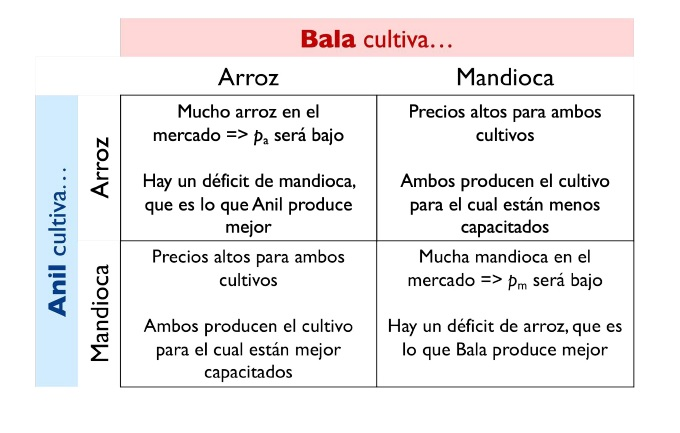
\includegraphics[scale=0.65]{Figures/Tema_03_7_bala.jpg}
\end{frame}

\begin{frame}
\frametitle{26. El juego de Anil y Bala}
\begin{itemize}
    \item Jugadores
        \begin{itemize}
        \item Anil y Bala, dos agricultores que deciden en qué cultivo especializarse
        \end{itemize}
    \item Estrategias viables
        \begin{itemize}
        \item Arroz o mandioca
        \end{itemize}
    \item Información
        \begin{itemize}
        \item Ningún agricultor sabe lo que el otro elige
        \end{itemize}
    \item Pagos
        \begin{itemize}
        \item Dependerá de los precios de mercado y de la calidad de la tierra
        \end{itemize}
\end{itemize}
\end{frame}

\begin{frame}
\frametitle{27. Construyendo la matriz de pagos}
\centering
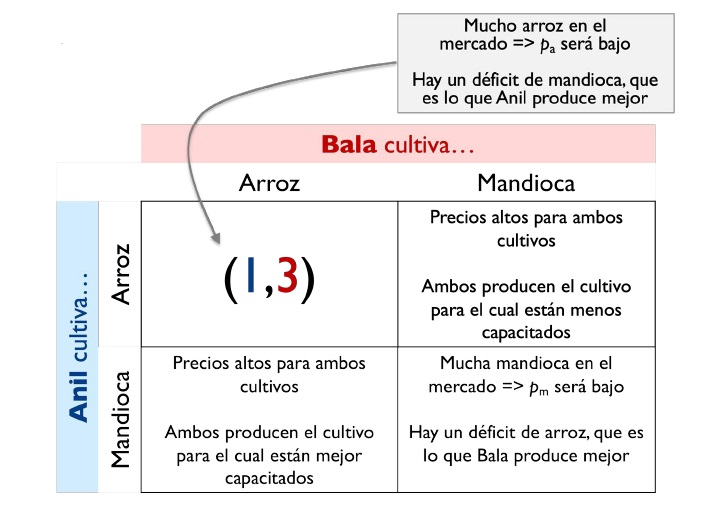
\includegraphics[scale=0.6]{Figures/Tema_03_8_bala.jpg}
\end{frame}

\begin{frame}
\frametitle{28. Construyendo la matriz de pagos}
\centering
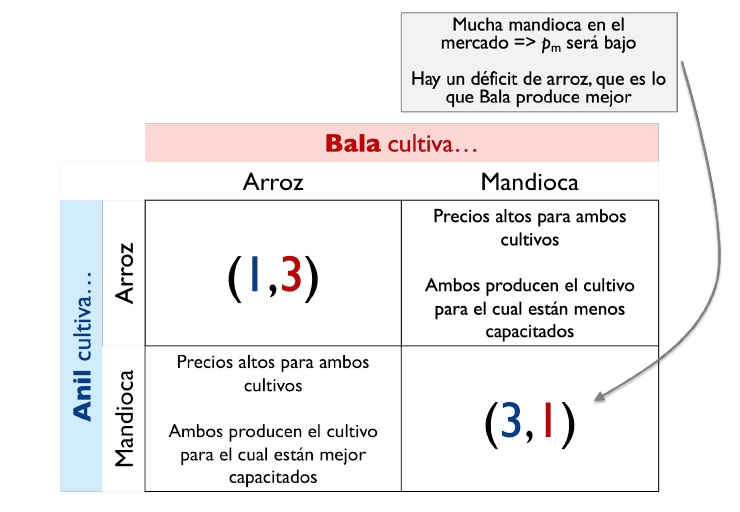
\includegraphics[scale=0.6]{Figures/Tema_03_9_bala.jpg}
\end{frame}

\begin{frame}
\frametitle{29. Construyendo la matriz de pagos}
\centering
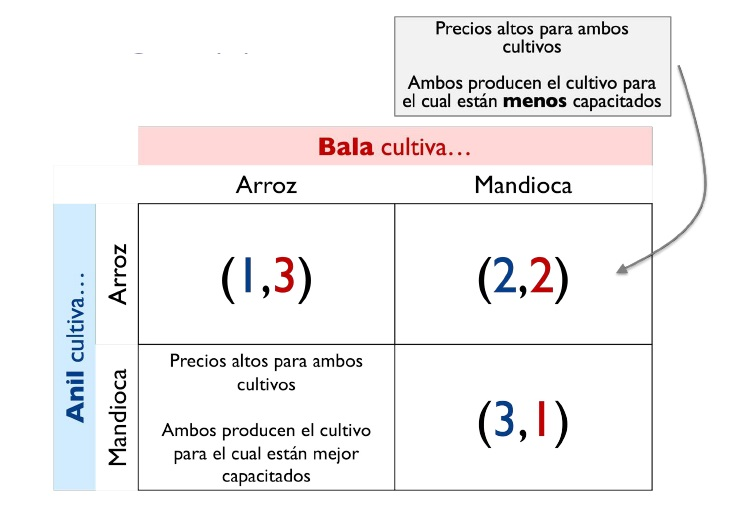
\includegraphics[scale=0.6]{Figures/Tema_03_10_bala.jpg}
\end{frame}

\begin{frame}
\frametitle{30. Construyendo la matriz de pagos}
\centering
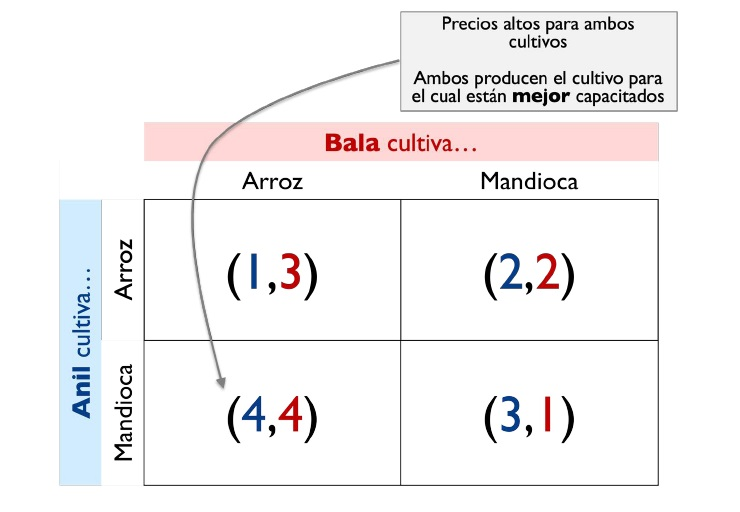
\includegraphics[scale=0.6]{Figures/Tema_03_11_bala.jpg}
\end{frame}

\begin{frame}
\frametitle{31. Matriz de pagos}
\centering
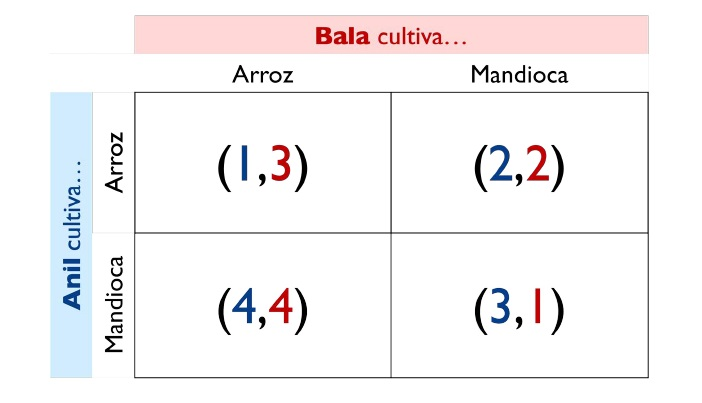
\includegraphics[scale=0.6]{Figures/Tema_03_12_bala.jpg}
\end{frame}

\begin{frame}
\frametitle{32. ¿Cómo pensamos el problema?}
\begin{itemize}
    \item ¿Cuál es la mejor respuesta de cada individuo?
        \begin{itemize}
        \item Aquella estrategia que brinda los mayores pagos, dada la estrategia seleccionada por la otra persona
        \end{itemize}
    \item A veces, existe una estrategia dominante
        \begin{itemize}
        \item Esta es una mejor respuesta a todas las posibles estrategias de otro jugador
        \end{itemize}
    \item Si se encuentra un resultado donde cada individuo juega su estrategia dominante, entonces nos encontramos con un equilibrio en estrategia dominante
\end{itemize}
\end{frame}

\begin{frame}
\frametitle{33. ¿Cómo piensa Anil?}
\centering
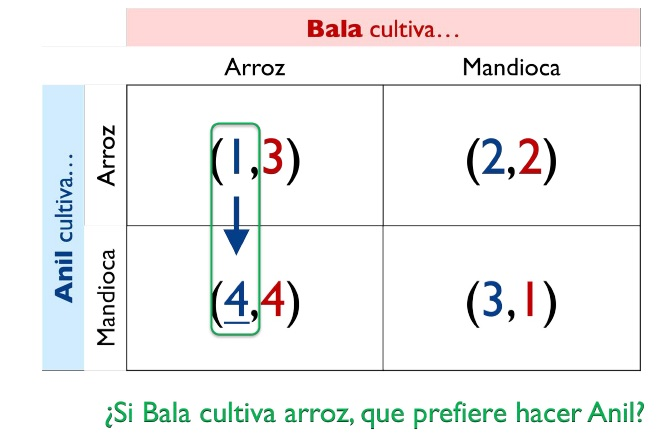
\includegraphics[scale=0.6]{Figures/Tema_03_13_bala.jpg}
\end{frame}

\begin{frame}
\frametitle{34. ¿Cómo piensa Anil?}
\centering
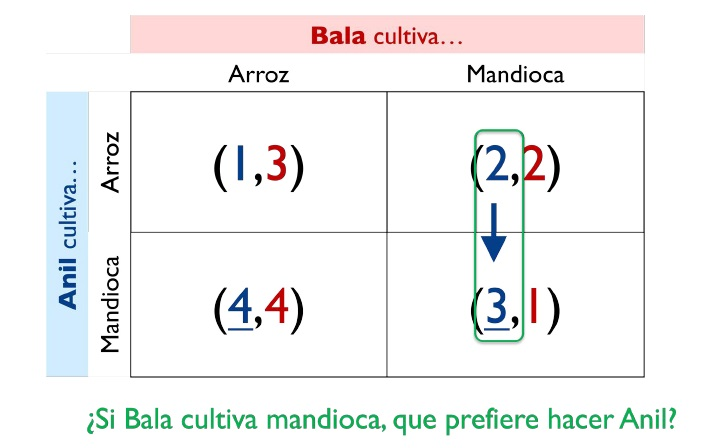
\includegraphics[scale=0.6]{Figures/Tema_03_14_bala.jpg}
\end{frame}

\begin{frame}
\frametitle{35. ¿Qué hace Anil?}
\centering
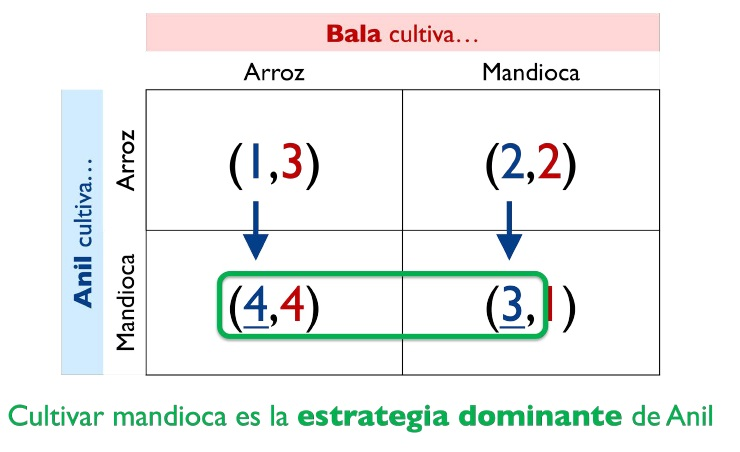
\includegraphics[scale=0.6]{Figures/Tema_03_15_bala.jpg}
\end{frame}

\begin{frame}
\frametitle{36. ¿Cómo piensa Bala?}
\centering
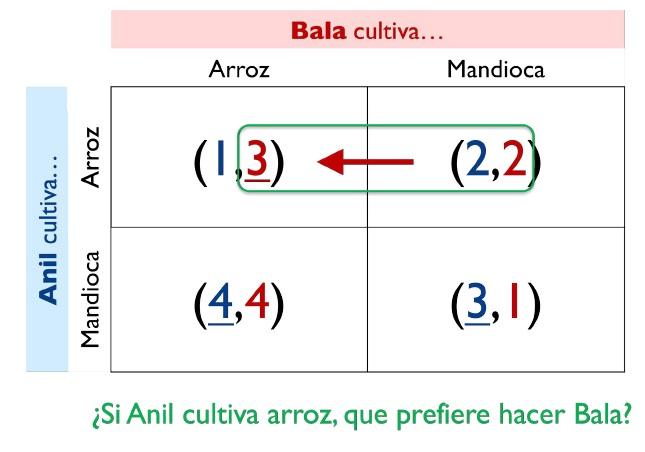
\includegraphics[scale=0.6]{Figures/Tema_03_16_bala.jpg}
\end{frame}

\begin{frame}
\frametitle{37. ¿Cómo piensa Bala?}
\centering
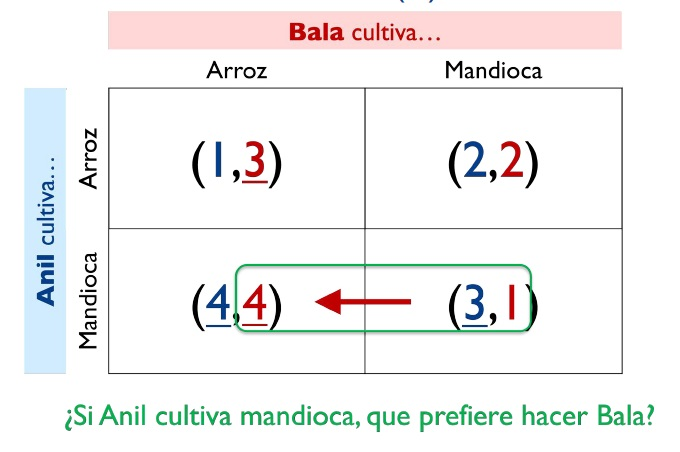
\includegraphics[scale=0.6]{Figures/Tema_03_17_bala.jpg}
\end{frame}

\begin{frame}
\frametitle{38. ¿Qué hace Bala?}
\centering
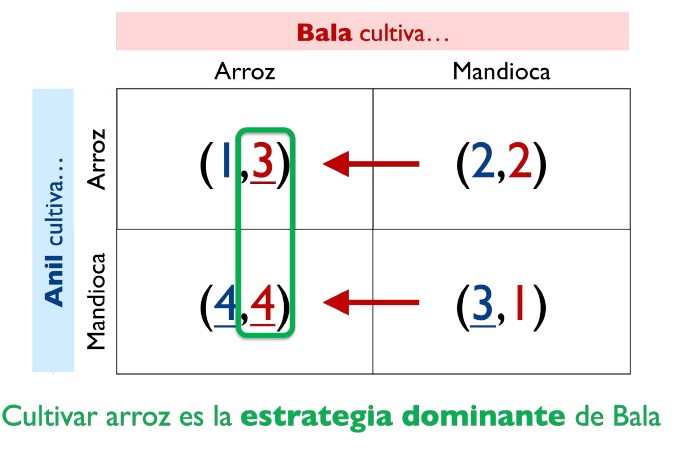
\includegraphics[scale=0.6]{Figures/Tema_03_18_bala.jpg}
\end{frame}

\begin{frame}
\frametitle{39. Equilibrio}
\centering
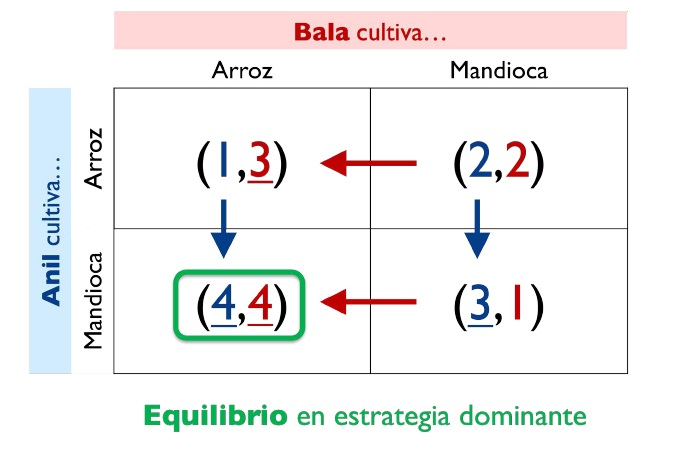
\includegraphics[scale=0.6]{Figures/Tema_03_19_bala.jpg}
\end{frame}

\begin{frame}
\frametitle{40. Otro juego}
\begin{itemize}
    \item Dos empresas productoras de \textit{smartphones}
    \item Comparten por igual el mercado de un país por, digamos, \$8 millones
    \item Enfrentan el problema de invertir en publicidad
        \begin{itemize}
        \item Si ambos invierten en publicidad, mantienen su proporción del mercado inalterada
        \item Si uno de ellos invierte  \$1 millón, se queda con $\frac{3}{4}$ del mercado
        \end{itemize}
    \item ¿Cómo analizamos este caso?    
\end{itemize}
\end{frame}

\begin{frame}
\frametitle{41. El juego de Apple y Samsung}
\begin{itemize}
    \item Jugadores
        \begin{itemize}
        \item Apple y Samsung, dos compañías que quieren maximizar su participación en el mercado
        \end{itemize}
    \item Estrategias viables
        \begin{itemize}
        \item Publicitar o no publicitar
        \end{itemize}
    \item Información
        \begin{itemize}
        \item Ambos tienen la misma información, y ninguno puede ver la decisión del otro antes de jugar
        \end{itemize}
    \item Pagos
        \begin{itemize}
        \item Dependerá del costo de publicidad y el mercado
        \end{itemize}
\end{itemize}
\end{frame}

\begin{frame}
\frametitle{42. Matriz de pagos}
\centering
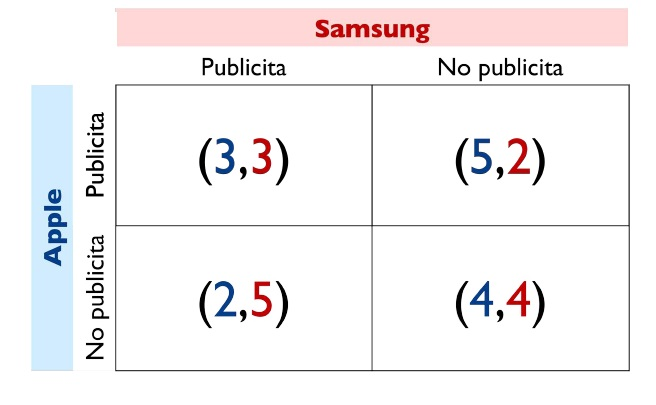
\includegraphics[scale=0.6]{Figures/Tema_03_20_bala.jpg}
\end{frame}

\begin{frame}
\frametitle{43. Equilibrio}
\centering
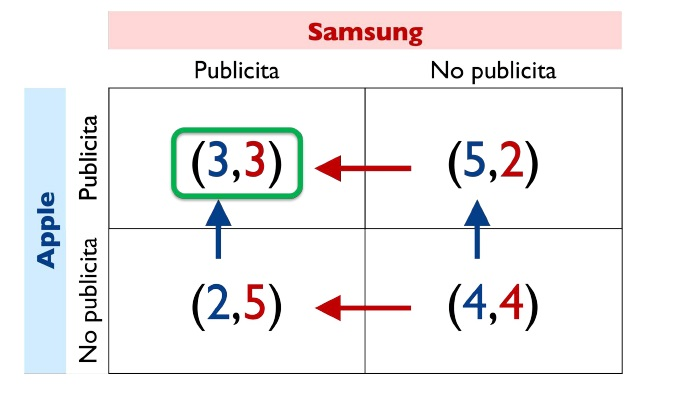
\includegraphics[scale=0.6]{Figures/Tema_03_21_bala.jpg}
\end{frame}

\begin{frame}
\frametitle{44. Dilema del prisionero}
\begin{itemize}
    \item Este ejemplo de las empresas de \textit{smartphones} es un dilema del prisionero disfrazado
        \begin{itemize}
        \item Típicamente, un juego con un equilibrio en estrategia dominante donde el resultado son pagos individuales y totales inferiores a otras estrategias posibles
        \end{itemize}
        \end{itemize}
        \textbf{El resultado socialmente óptimo no es alcanzado} \vspace{2mm}
        \begin{itemize}
        \item Este tipo de dilema es útil para representar una serie de problemáticas sociales
        \begin{itemize}
        \item Desde temas ambientales hasta conflictos en la provisión de algunos tipos de bienes
        \end{itemize}
\end{itemize}
\end{frame}

\begin{frame}
\frametitle{45. Problemas y soluciones}
\begin{itemize}
    \item ¿Por qué se llega a este tipo de resultado y en qué forma se puede amenorar o solucionar?
    \item Algunas razones (y soluciones)
        \begin{itemize}
        \item Los jugadores sólo se preocupan por sus propios beneficios \\
        - Podemos introducir preferencias sociales
        \item Nadie puede hacer que los jugadores paguen por las consecuencias de sus acciones sobre los demás \\
        - Juegos repetidos, normas sociales y castigo de pares
        \item Los jugadores no pueden coordinar sus acciones con antelación \\
        - Cambiar las reglas del juego (instituciones y políticas)
        \end{itemize}
\end{itemize}
\end{frame}

\begin{frame}
\frametitle{46. Asfaltando la calle}
\begin{itemize}
    \item Dos familias viven en una calle de tierra (Álvarez y Benítez)
    \item Ambas se beneficiarían si se asfaltara la calle
        \begin{itemize}
        \item Por ejemplo, tendrían que gastar menos en arreglo y limpieza de sus autos por \$15.000
        \end{itemize}
    \item Enfrentan el problema de invertir en el asfalto
        \begin{itemize}
        \item El costo de asfaltar la calle es de \$20.000
        \item Puede pagarlo una u otra familia, o las dos juntas
        \end{itemize}
\item ¿Cómo analizamos este caso?
\end{itemize}
\end{frame}

\begin{frame}
\frametitle{47. El juego del asfalto}
\begin{itemize}
    \item Jugadores
        \begin{itemize}
        \item Familias Álvarez y Benítez
        \end{itemize}
    \item Estrategias viables
        \begin{itemize}
        \item Pagar o no pagar por el asfalto
        \end{itemize}
    \item Información
        \begin{itemize}
        \item Ambos tienen la misma información, y ninguno puede ver la decisión del otro antes de jugar
        \end{itemize}
    \item Pagos
        \begin{itemize}
        \item Dependerá del ahorro en arreglos del auto y la contribución al costo del asfalto
        \end{itemize}
\end{itemize}
\end{frame}

\begin{frame}
\frametitle{48. Pagando por el asfalto}
\centering
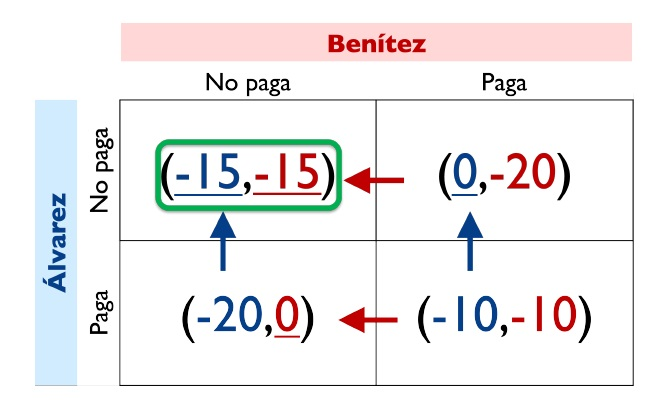
\includegraphics[scale=0.6]{Figures/Tema_03_27_abel.jpg}
\end{frame}

\begin{frame}
\frametitle{49. El problema del bien público}
\begin{itemize}
    \item Existe un tipo de bien, usualmente llamado bien público, con dos características distintivas:
    \begin{itemize}
        \item Es no rival \\
        - Su uso por una persona no perjudica o impide el uso simultáneo por parte de otros individuos
        \item Es no excluyente \\
        - No se puede impedir ser utilizado
    \end{itemize}
    \item El dilema del prisionero ilustra un problema de los bienes públicos: pueden no producirse
    \begin{itemize}
        \item Dadas sus característica, existe la posibilidad de hacer free-riding \\
        - ¡No contribuir es la estrategia dominante!
    \end{itemize}
\end{itemize}
\end{frame}

\begin{frame}
\frametitle{50. Pagando por los costos que uno genera}
\begin{itemize}
    \item Tanto en el caso del asfalto, como en el de los pesticidas elaborado en “The Economy”: \\
\end{itemize}
\vspace{5mm}
\textbf{Es difícil hacer pagar a los jugadores por la
consecuencias de sus acciones sobre los demás}
\end{frame}

\begin{frame}
\frametitle{51. Mitigando el problema}
\begin{itemize}
    \item Mecanismos ayudan a reducir el problema
    \begin{itemize}
        \item Juegos repetidos \\
        - Repetición contribuye a la cooperación: las consecuencias en el futuro hacen la estrategia egoísta sub-óptima
        \item Normas sociales \\
        - Reglas que indican como actuar en contextos particulares \\
        - Individuos a veces incurren en considerables costos para castigar a pares que violan normas sociales o llevan a cabo acciones que consideran injustas (¿gusto por equidad?)
    \end{itemize}
\end{itemize}
\end{frame}

\begin{frame}
\frametitle{52. Aprendiendo sobre preferencias}
\begin{itemize}
    \item Los economistas utilizan a veces experimentos para aprender sobre las preferencias
    \begin{itemize}
        \item En el laboratorio: \\
        - Se puede controlar las decisiones de los participantes y sus resultados \\
        - Se puede crear un grupo de control / tratamiento para la comparación \\
        - Los resultados pueden ser replicados \\
        - Se pueden controlar otras variables
        \item En el campo \\
        - Algunos experimentos de laboratorio no pueden predecir la toma de decisiones en el mundo real \\
        - El campo provee un contexto más realista en el que las personas toman decisiones
    \end{itemize}
\end{itemize}
\end{frame}

\begin{frame}
\frametitle{53. El dilema de la guardería}
\begin{itemize}
    \item Un experimento `real' (`field experiment')
       \begin{itemize}
       \item Se introdujo una multa a la llegada tarde de los padres... con un resultado no esperado \\
        - ¡Más padres empezaron a llegar tarde!
        \end{itemize}
    \item ¿Por qué?
        \begin{itemize}
        \item Antes del experimento, llegar tarde era `incorrecto' 
        \item El tiempo de los maestros pasó a tener un valor definido \\
        - El precio del retardo, que los padres podían estar dispuestos a pagar o no \\ 
        \item En este caso, se dice que los incentivos hicieron un crowding out de las preferencias sociales
    \end{itemize}
\end{itemize}
\end{frame}

\begin{frame}
\frametitle{54. En el campo ... con padres y niños}
\centering
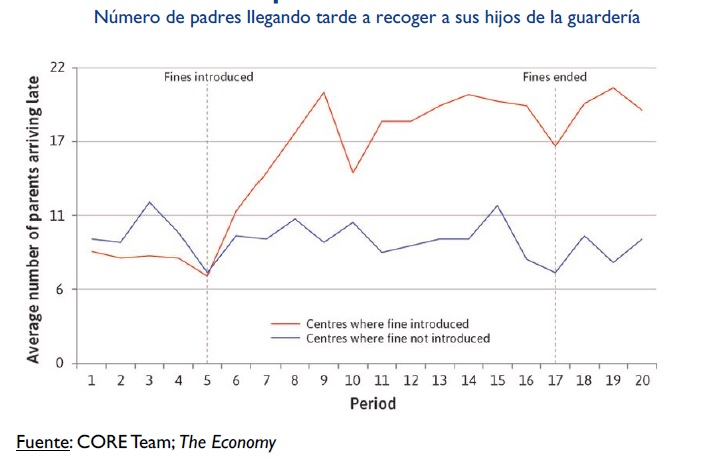
\includegraphics[scale=0.6]{Figures/Tema_03_28_guarderia.jpg}
\end{frame}

\begin{frame}
\frametitle{55. Negociando}
\begin{itemize}
    \item La cooperación es posible aun cuando agentes 
    actúan en forma independiente
    \begin{itemize}
        \item En muchos de los ejemplos que discutimos no fue necesario que los individuos se pusieran de acuerdo \\
        - A veces las condiciones del juego ayudaban (con Anil y Bala), o si se repetía el juego, o si permitía sancionar a los que no colaboraban
    \end{itemize}
    \item Pero la negociación es otra herramienta para conseguir un acuerdo mutuamente beneficioso
    \begin{itemize}
        \item Más fácil decirlo que hacerlo \\
        - ¿Cómo repartir los costos y beneficios de la interacción?
    \end{itemize}
\end{itemize}
\end{frame}

\begin{frame}
\frametitle{56. Motivando preferencias sociales}
\begin{itemize}
        \item Altruismo
        \begin{itemize}
            \item Una persona puede ser altruista y preocuparse de la felicidad (o sobre algún otro aspecto del bienestar) de los demás
        \end{itemize}
        \item Equidad
        \begin{itemize}
            \item La importancia de distribuir recursos en forma justa \\
            - Motivación por lo que los economistas llaman `aversión por la desigualdad'
        \end{itemize}
        \item Reciprocidad
        \begin{itemize}
            \item Existencia de preferencias recíprocas \\
            - Si en el pasado han sido generosos con nosotros, merecemos tratar en forma generosa
        \end{itemize}
\end{itemize}
\end{frame}

\begin{frame}
\frametitle{57. Juego del ultimátum}
\begin{itemize}
        \item Una herramienta muy utilizada para estudiar preferencias sociales es el juego del ultimátum
        \begin{itemize}
            \item ü Dos jugadores, seleccionados aleatoriamente \\ 
            - Proponente \\
            - Receptor
            \item El proponente recibe algo de valor (típicamente dinero) y debe ofrecerle al receptor una parte \\
            - Que puede ser cualquier cosa entre todo y nada \\
            - El receptor sabe cuán grande es el total
            \item Una vez que el receptor escucha la oferta, decide si la acepta o no \\
            - Si la oferta es rechazada, nadie recibe nada \\
            - Si es aceptada, se reparte como sugirió el proponente
        \end{itemize}
\end{itemize}
\end{frame}

\begin{frame}
\frametitle{58. Juego secuencial}
\centering
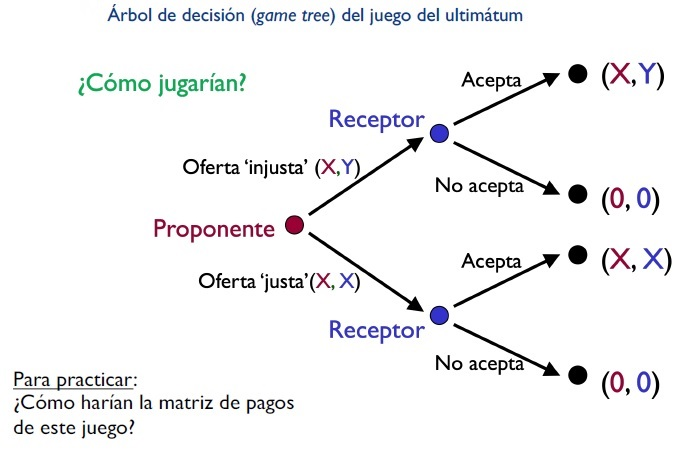
\includegraphics[scale=0.6]{Figures/Tema_03_29_arbol.jpg}
\end{frame}

\begin{frame}
\frametitle{59. Agricultores versus estudiantes}
\centering
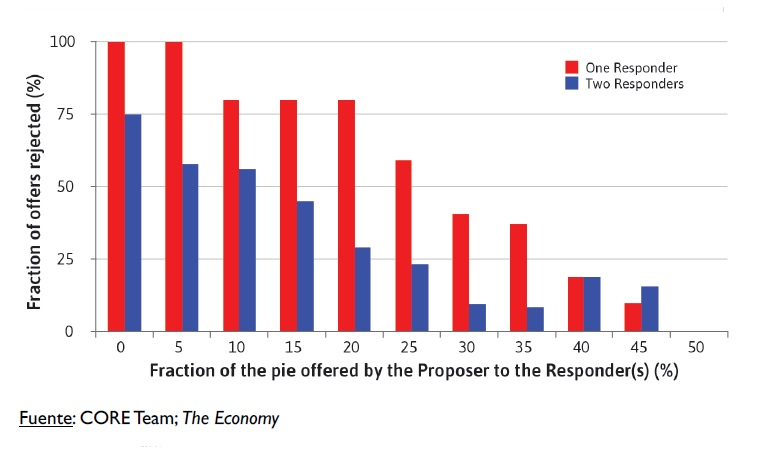
\includegraphics[scale=0.6]{Figures/Tema_03_32_ultimatum.jpg}
\end{frame}

\begin{frame}
\frametitle{60. ¿Cuál es el beneficio esperado?}
\centering
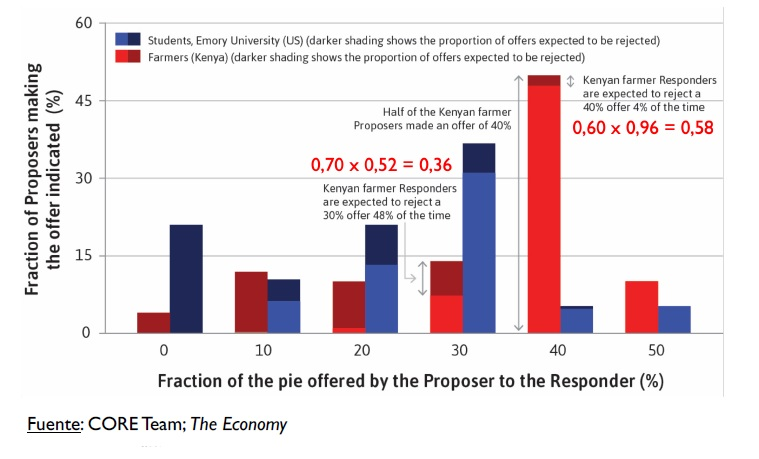
\includegraphics[scale=0.6]{Figures/Tema_03_31_ultimatum.jpg}
\end{frame}

\begin{frame}
\frametitle{61. ¿Y si hay competencia?}
\centering
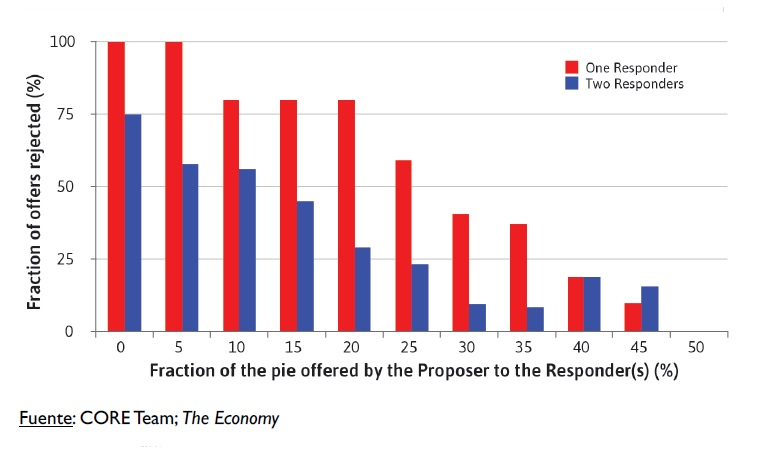
\includegraphics[scale=0.6]{Figures/Tema_03_32_ultimatum.jpg}
\end{frame}

\begin{frame}
\frametitle{62. Equilibrio de Nash}
\begin{itemize}
        \item Hasta ahora, siempre encontramos un equilibrio en estrategias dominantes
        \begin{itemize}
            \item Existía una estrategia dominante para los jugadores
        \end{itemize}
        \item Existe otro concepto de equilibrio que suele ser útil, el equilibrio de Nash
        \end{itemize}
\textbf{Resultado de un juego donde ninguno de los jugadores desea jugar de manera distinta, dadas las acciones de cada uno de los demás jugadores} \vspace{2mm}
\begin{itemize}
        \begin{itemize}
            \item Cada jugador ha adoptado su mejor estrategia \\
            - Por lo cual, ningún jugador gana cambiando su estrategia si nadie más cambia la suya
        \end{itemize}
        \end{itemize}
\end{frame}

\begin{frame}
\frametitle{63. La batalla de los sexos}
\begin{itemize}
        \item Una pareja arregló para ir al cine
        \begin{itemize}
            \item Alberto y Beatriz
        \end{itemize}
        \item No recuerdan qué película iban a ver
        \begin{itemize}
            \item Alberto quería ir a ver una comedia romántica
            \item Beatriz una de acción
        \end{itemize}
        \item Ambos prefieren ir al mismo lugar que desencontrarse
        \item No tienen forma de comunicarse
        \item ¿Cómo analizamos este caso?
\end{itemize}
\end{frame}

\begin{frame}
\frametitle{64. ¿Y si hay competencia?}
\centering
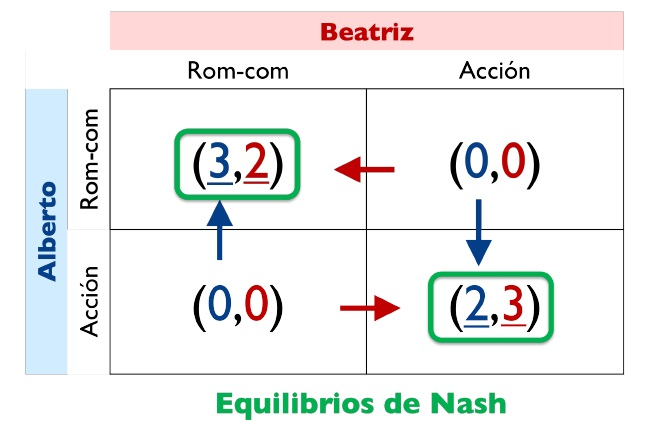
\includegraphics[scale=0.6]{Figures/Tema_03_33_batallasexo.jpg}
\end{frame}

\begin{frame}
\frametitle{65. Juegos de coordinación}
\begin{itemize}
        \item La batalla de los sexos es un típico juego de coordinación
        \begin{itemize}
            \item Ilustra situaciones que encontramos por doquier en la sociedad \\
            - ¿Qué plataforma de social media usar? ¿De qué lado del camino conducir?
        \end{itemize}
        \item En este caso, el pago era idéntico en ambos equilibrios, pero puede que los jugadores queden atrapados en un mal equilibrio
        \begin{itemize}
            \item ¿Cómo se decide, por ejemplo, pasar de una tecnología a otra cuando la nueva implica un costo para el capitalista y para el trabajador?
        \end{itemize}
\end{itemize}
\end{frame}

\begin{frame}
\frametitle{66. Juegos de coordinación}
\begin{itemize}
        \item La batalla de los sexos es un típico juego de coordinación
        \begin{itemize}
            \item Ilustra situaciones que encontramos por doquier en la sociedad \\
            - ¿Qué plataforma de social media usar? ¿De qué lado del camino conducir?
        \end{itemize}
        \item En este caso, el pago era idéntico en ambos equilibrios, pero puede que los jugadores queden atrapados en un mal equilibrio
        \begin{itemize}
            \item ¿Cómo se decide, por ejemplo, pasar de una tecnología a otra cuando la nueva implica un costo para el capitalista y para el trabajador?
        \end{itemize}
\end{itemize}
\end{frame}

\begin{frame}
\frametitle{67. Inversión en nueva tecnología}
\begin{itemize}
        \item Dos tipos de agente en la economía
        \begin{itemize}
            \item Capitalistas y trabajadores
        \end{itemize}
        \item Se está considerando introducir una nueva tecnología
        \begin{itemize}
            \item Ésta aumenta la productividad del trabajador y permite al capitalista producir a un menor costo
        \end{itemize}
        \item La tecnología no es gratuita para ninguno
        \begin{itemize}
            \item El costo del capital para el capitalista
            \item La inversión en capital humano para el trabajador
        \end{itemize}
        \item ¿Cómo analizamos este caso?
\end{itemize}
\end{frame}

\begin{frame}
\frametitle{68. Cambio tecnológico}
\centering
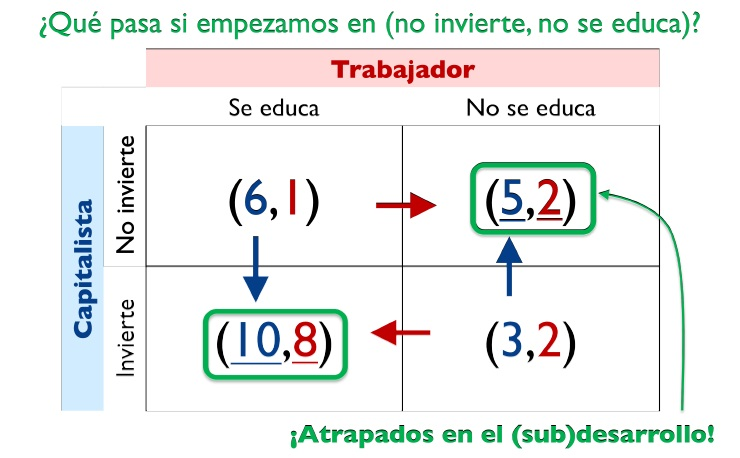
\includegraphics[scale=0.6]{Figures/Tema_03_34_catecno.jpg}
\end{frame}

\end{document}
